\documentclass[headings=standardclasses, abstract=true]{scrartcl}

\usepackage{graphicx} % Required for inserting images
\usepackage[sorting=none, style=science]{biblatex} % Required for bibliography
\usepackage{amsmath} % For math equations
\usepackage{minted} % For code blocks
\usepackage[framemethod=TikZ]{mdframed} % For code blocks
\usepackage[svgnames]{xcolor} % For colors
\usepackage{fontspec} % For custom fonts
\usepackage{caption} % For subfigures
\usepackage{subcaption} % For subfigures
\usepackage{float}
\usepackage[
    top=3cm,
    bottom=3cm,
    left=3cm,
    right=3cm
]{geometry} % Required for setting the page size
\usepackage[
    pdfauthor={Sina Atalay, Sacha Escudier, Kentaro Hanson},
    pdftitle={FastFEM v0.0.1},
    hidelinks=true
]{hyperref} % Required for hyperlinks and metadata

% Path to the bibliography file:
\addbibresource{../docs/assets/bibliography.bib}

% For Python blocks:
\newmdenv[
    outerlinewidth=1,
    outerlinecolor=Gainsboro,
    middlelinewidth=0,
    backgroundcolor=GhostWhite,
    roundcorner=3pt,
    innerbottommargin=12pt,
    innertopmargin=12pt,
    innerleftmargin=12pt,
    innerrightmargin=12pt,
    skipbelow=-0pt
]{pythonbox}
\newfontfamily\vscodefont{Droid Sans Mono}[NFSSFamily=VSCode]
\newcommand{\pythonCodeBlock}[3]{%
    \begin{figure}
        \centering
        \begin{pythonbox}
            \inputminted[fontfamily=VSCode, fontsize=\scriptsize]{python}{#1}
        \end{pythonbox}
        \caption{#2}
        \label{#3}
    \end{figure}
}


\title{\texttt{FastFEM v0.0.1}}
\subtitle{
    A Python package for solving PDEs with the finite element method    \\
    \vspace{0.2cm}
    \href{https://fastfem.com}{fastfem.com}
}
\author{
    Sina Atalay\textsuperscript{1*}, Sacha Escudier\textsuperscript{1*}, Kentaro Hanson\textsuperscript{1*} \\
    {\footnotesize \textsuperscript{1}Princeton University, Princeton, NJ, USA}\\
    {\footnotesize \textsuperscript{*}All authors contributed equally}
}
\date{
    \normalsize December 2024
}


\begin{document}

\maketitle

\begin{abstract}
\noindent Lorem ipsum dolor sit amet, consectetur adipiscing elit. Vestibulum congue gravida sem non dictum. Aenean sit amet mi fermentum ante laoreet dictum sit amet a magna. Praesent sed aliquet dui. Vivamus scelerisque condimentum mauris id euismod. Duis elementum urna eu rutrum mattis. Donec fermentum, risus et viverra aliquet, ante sapien consequat augue, sit amet dictum est nisl id elit. Proin dapibus congue tincidunt. Pellentesque habitant morbi tristique senectus et netus et malesuada fames ac turpis egestas. Fusce felis eros, aliquam sed dui ut, tempor condimentum neque. Donec quis sapien bibendum, faucibus urna sed, gravida felis. Praesent et quam ligula. Aliquam ac est eu odio tincidunt volutpat a in augue. Maecenas fermentum velit felis, vel viverra dui scelerisque pharetra. Nullam eros lorem, finibus pulvinar eleifend eu, pulvinar ac ipsum. Sed velit neque, venenatis sit amet urna vitae, vulputate ullamcorper est.
\end{abstract}

\section{Introduction}

Partial differential equations (PDEs) are the fundamental tools for mathematically modeling natural phenomena. Many fundamental phenomena observed in nature, such as general relativity\supercite{Marolf2001}, quantum mechanics \supercite{Feit1982}, heat diffusion\supercite{Bergman2011}, fluid mechanics\supercite{Lukaszewicz2016}, pricing of financial derivative contracts\supercite{Barles1998}, structural analysis\supercite{Boresi2002}, and electromagnetism\supercite{Griffiths2017}, are described by PDEs. However, most of these PDEs do not have closed-form solutions, especially in complex geometries. Therefore, engineers have developed many numerical methods for solving PDEs. One of the most popular numerical methods among them is the finite-element method (FEM), which originated in the early 1940s\supercite{Liu2022}. FEM is capable of solving non-linear PDEs in highly complex geometries. Since the 1940s, FEM has undergone significant advancements and has revolutionized the way scientific modeling and engineering design. Today, it is widely used in many industrial applications.

Currently, there are many open-source FEM software out there\supercite{fem_getdp, fem_agros, fem_calculix, fem_elmerfem, fem_freefem, fem_goma, fem_fenicsx, fem_dealii}. With \texttt{FastFEM}\supercite{fastfem}, we attempt to develop another open-source FEM software package with the goal of

\begin{itemize}
    \item Creating an easy-to-use and clean Python interface
    \item Using modern tools like JAX\supercite{jax2018github} for advanced array computing with automatic differentiation capabilities
\end{itemize}

One of the motivations for creating a Python interface was the capability of the language to create very intuitive-to-use interfaces. A modern Python interface can offer users a great way of describing FEM problems. The other motivation was leveraging the existing scientific Python environment. Python's popularity in the scientific world is still increasing, and modern libraries with state-of-the-art technologies like JAX, PyVista\supercite{Sullivan2019}, etc., are being developed.


FastFEM is planned to be a big project, but as the goal of \texttt{v0.0.1}, we decided to focus on 2D parabolic PDEs. Parabolic PDEs, such as the heat diffusion equation, Poisson's equation, and the Black-Scholes equation, are very common in various applications. A 2-dimensional parabolic PDE can be expressed as

\begin{equation}
    \frac{\partial^2 f(x,y,t)}{\partial x^2} + \frac{\partial^2 f(x,y,t)}{\partial y^2}
    =
    h(f) \frac{\partial f(x,y,t)}{\partial t} + g(x,y)
    \label{pde}
\end{equation}
where $f(x,y,t)$, $h(f)$, and $g(x,y)$ are scalar functions, $x$ and $y$ are spatial coordinates, and $t$ is time.

Currently, \texttt{FastFEM v0.0.1} can
\begin{enumerate}
    \item create a 2D mesh,
    \item take initial conditions, boundary conditions, h(f), and g(x,y) as inputs,
    \item solve \autoref{pde} with FEM, and
    \item plot the solution.
\end{enumerate}


In this report, the theory behind FEM is summarized. The features and capabilities of \texttt{FastFEM v0.0.1} are presented. Some example results are shown. Finally, the conclusion and outlook are discussed.

\section{Theory}

TODO: when filling this section, please note that these equations are referenced outside this section. You can change the equation (function labels/etc, like if you want to use a different symbol than $K$ for the stiffness) if you perfer a different format, but the main idea should stay the same.



\begin{equation}
    M(\phi_i,\phi_j) = \int_{\Omega}\phi_i \phi_j~dV
    \label{eqn:mass_matrix}
\end{equation}

\begin{equation}
    K(\phi_i,\phi_j) = \int_{\Omega}(\nabla\phi_i)\cdot (\nabla\phi_j)~dV
    \label{eqn:stiffness_matrix}
\end{equation}


\section{Features and Capabilities}

This section summarizes \texttt{FastFEM v0.0.1}'s features and capabilities: mesh generation, solving parabolic PDEs with FEM using elements and fields, and plotting.

\subsection{Mesher}

\texttt{FastFEM} uses Gmsh\supercite{Gmsh} for mesh generation. Currently, \texttt{v0.0.1} offers two fundamental 2D mesh generation functions, as shown in \autoref{fig:mesh-example1}.  The results of the functions are shown in \autoref{fig:mesh}. \texttt{FastFEM} is fully statically typed so that users can get autocomplete suggestions when writing the function's arguments and using the mesh object it returns.

\pythonCodeBlock{figures/mesher-example1.py}{Two available functions of \texttt{FastFEM v0.0.1} for generating 2D square and rectangle meshes that are shown in \autoref{fig:mesh}.}{fig:mesh-example1}

\begin{figure}[H]
    \centering
    \hfill
    \begin{subfigure}[c]{0.4\textwidth}
        \centering
        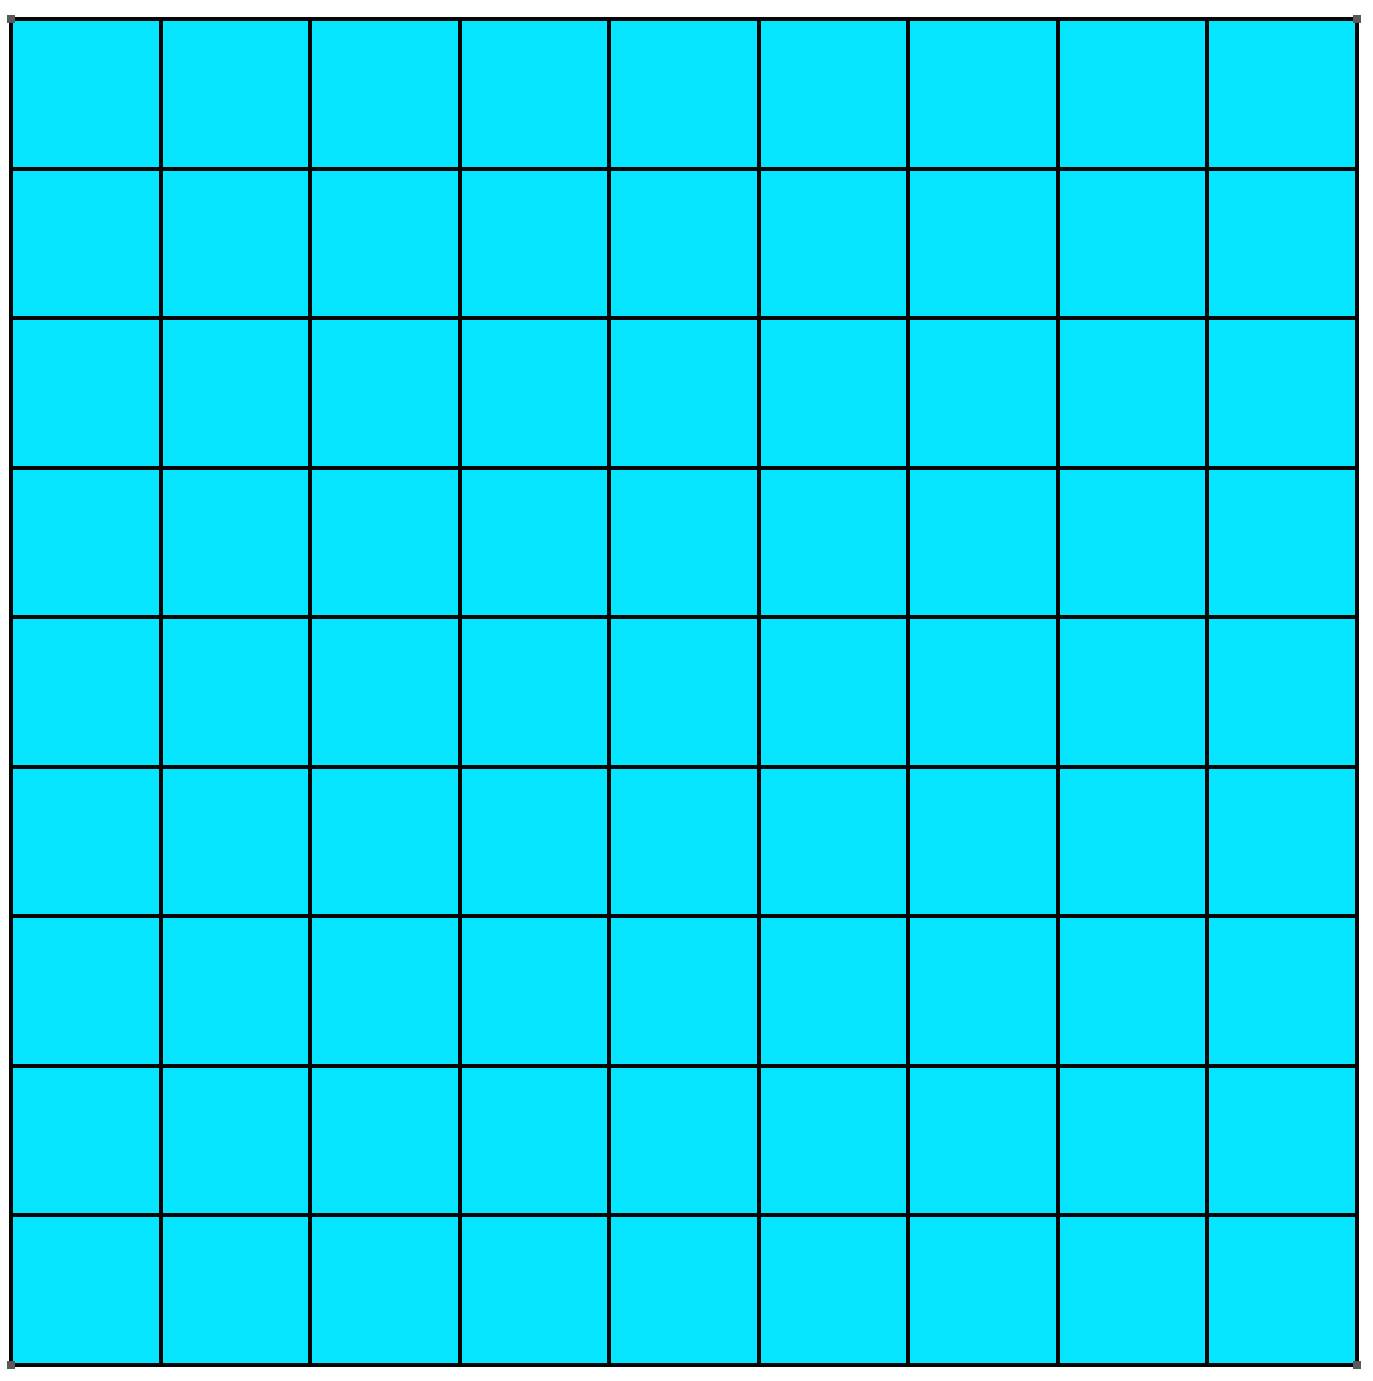
\includegraphics[width=\textwidth]{figures/square_mesh.png}

        \caption{Square mesh.}
        \label{fig:square}
    \end{subfigure}
    \hspace{0.1\textwidth}
    \begin{subfigure}[c]{0.4\textwidth}
        \centering
        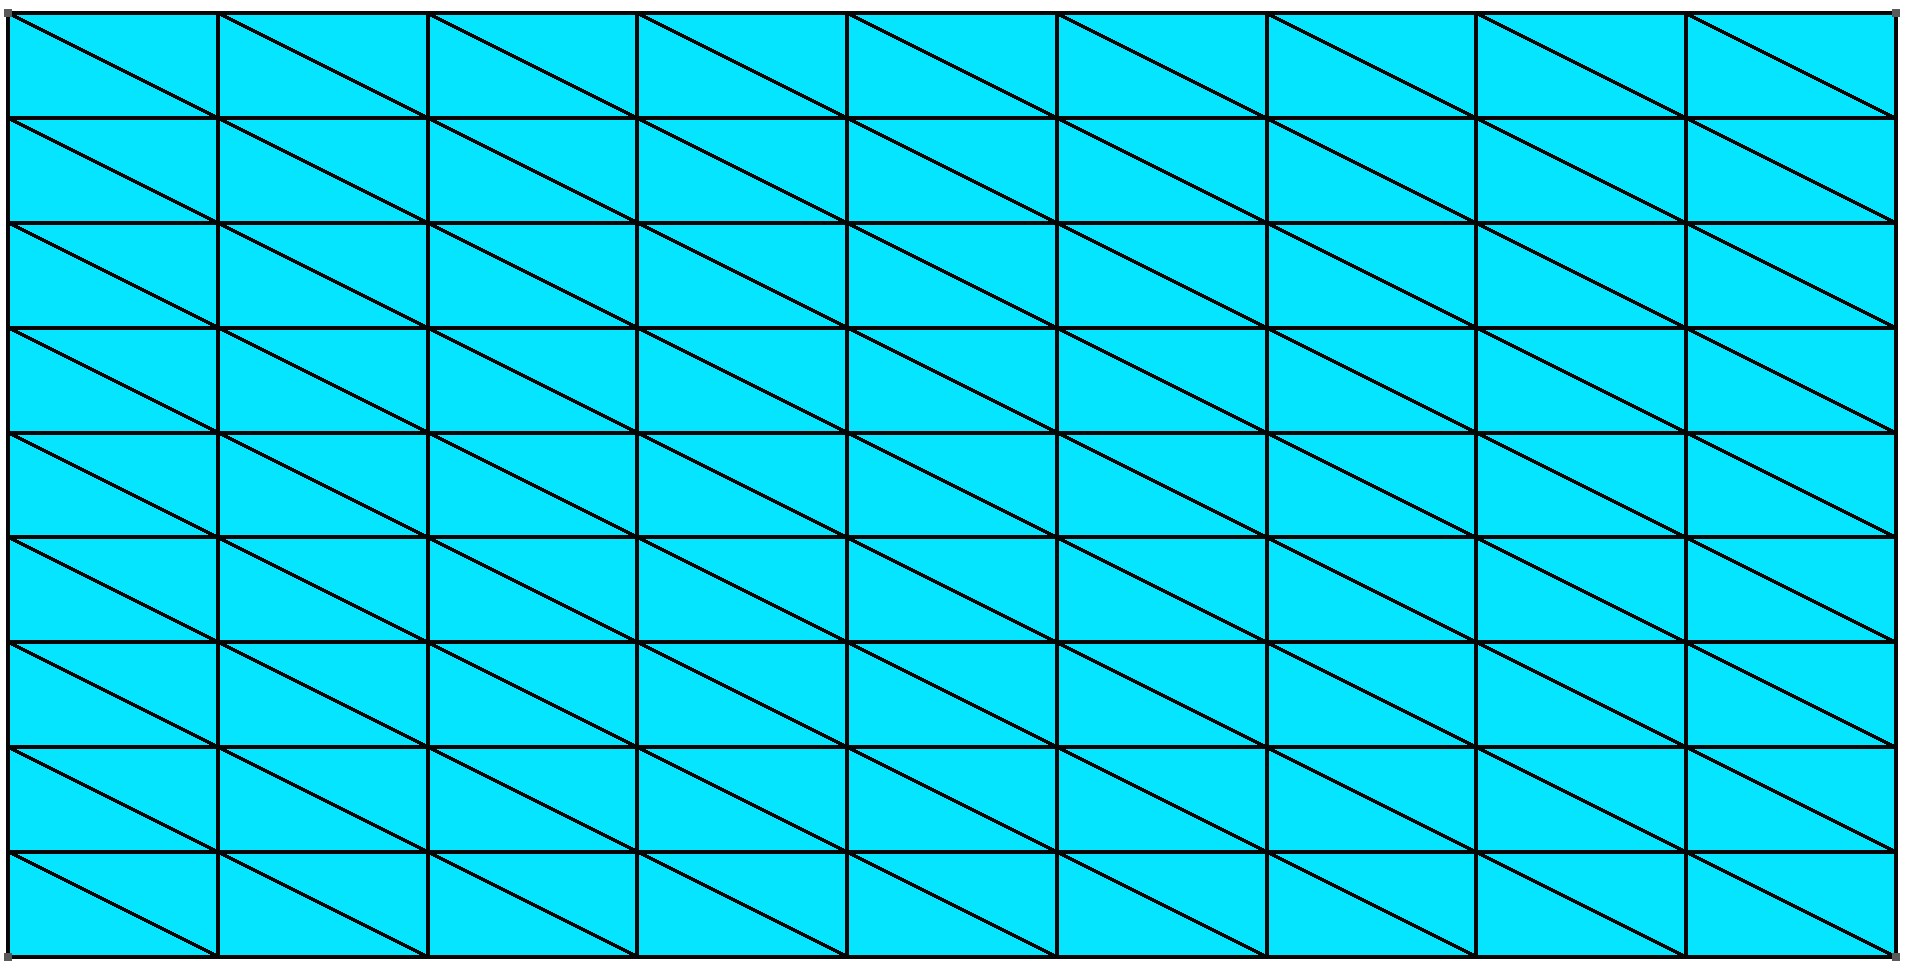
\includegraphics[width=\textwidth]{figures/rectangle_mesh.png}
        \caption{Rectangle mesh.}
        \label{fig:rectangle}
    \end{subfigure}
    \caption{Two examples of mesh generated with the functions in \autoref{fig:mesh-example1}.}
    \label{fig:mesh}
    \hfill
\end{figure}

\texttt{FastFEM v0.0.1} also provides a general-purpose, object-oriented interface for 2D mesh generation by abstracting Gmsh's functional approach. For example, a mesh of an arbitrary 2D geometry, as shown in \autoref{fig:arbitrarymesh}, can be created using the code presented in \autoref{fig:mesh-example2}.

\pythonCodeBlock{figures/mesher-example2.py}{The code that generates the mesh of an arbitrary geometry shown in \autoref{fig:arbitrarymesh}.}{fig:mesh-example2}

\begin{figure}[H]
    \centering
    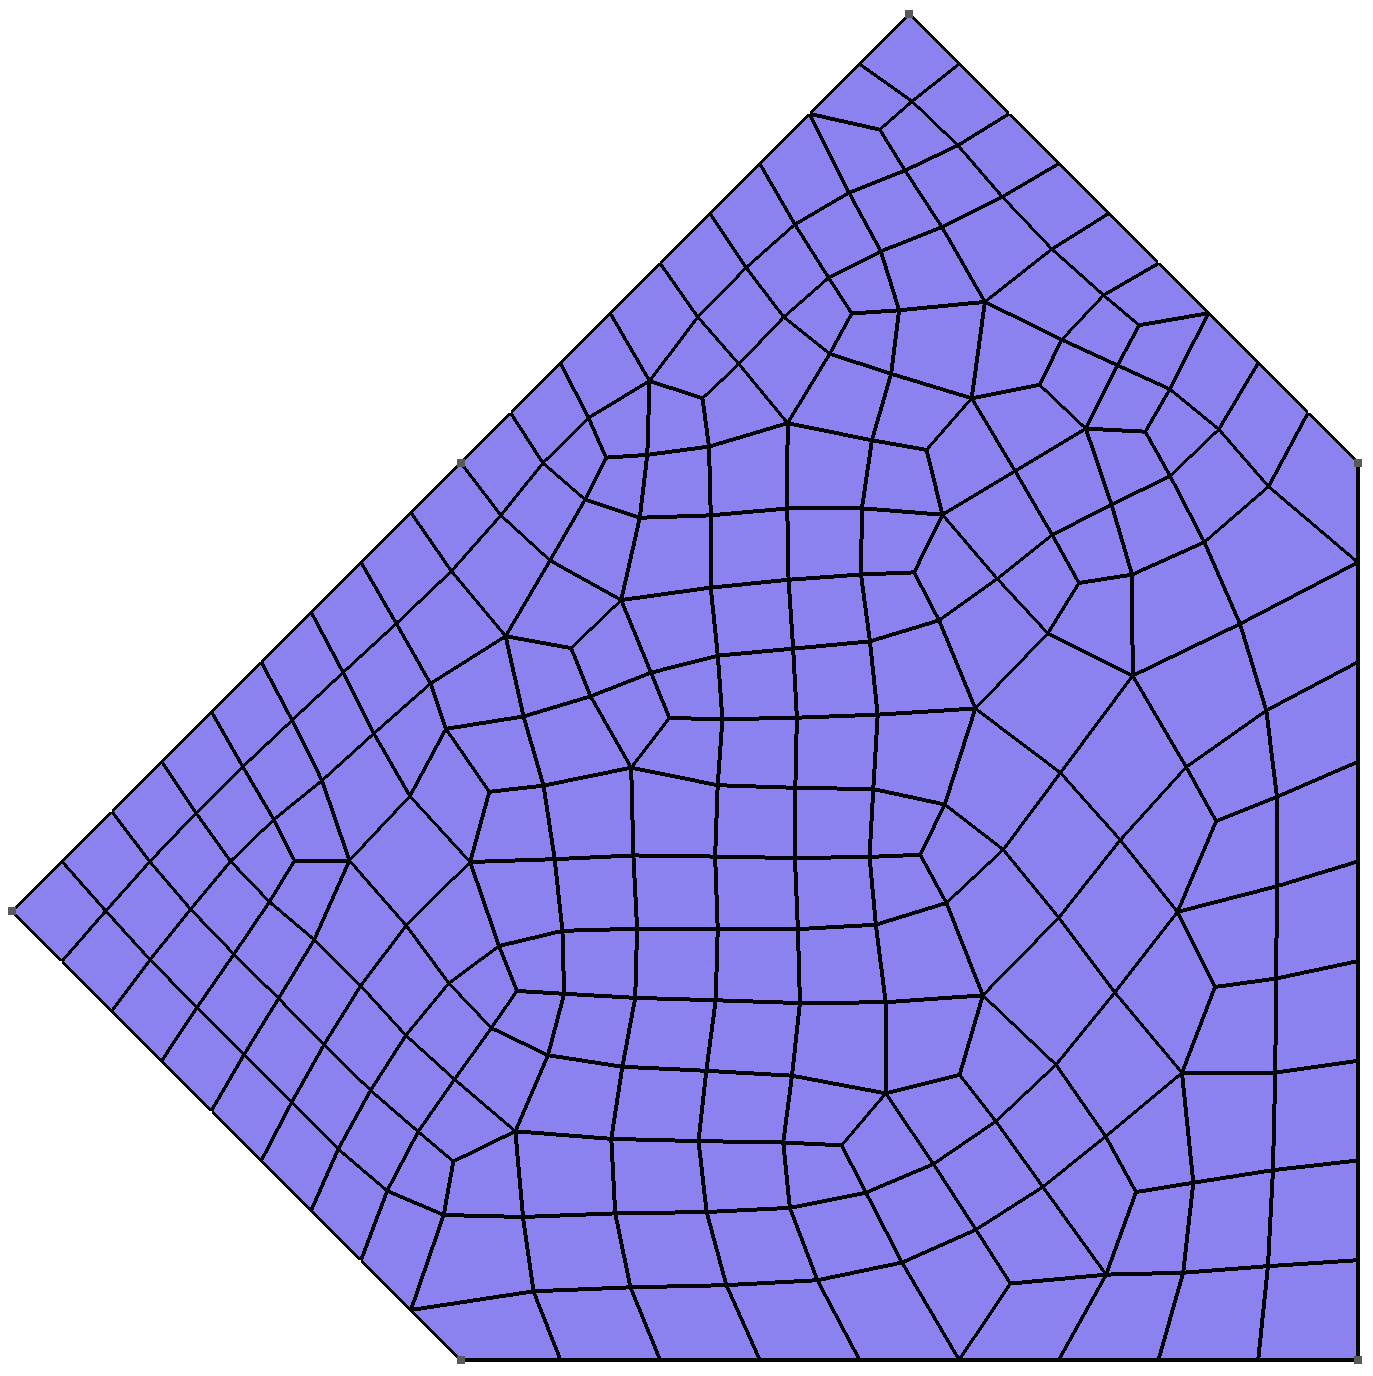
\includegraphics[width=0.5\textwidth]{figures/arbitrary_mesh.png}
    \caption{An arbitrary 2D mesh generated using the code in \autoref{fig:mesh-example2}.}
    \label{fig:arbitrarymesh}
\end{figure}

\subsection{Elements and Fields}
In order to use the weak formulation, \texttt{FastFEM} needs to know how to integrate functions on a given mesh. Each element type specifies both the shape functions and the algorithm used to integrate a function on that element. For example, the mass matrix entries (\ref{eqn:mass_matrix}) on two different element types are:

\begin{itemize}
\item For linear triangular elements with shape functions $\{\phi_1,\phi_2,\phi_3\}$ having the Kronecker delta property for each vertex ($\phi_i(v_j) = \delta_{ij}$ for vertices $v_1,v_2,v_3$), the analytical solution to the integral is known, since the shape functions are linear.

\item Spectral elements, a technique used in fluid dynamics (Patera 1984)\supercite{Patera1984} and other continuum mechanical fields, have shape functions $\phi_{i_1,i_2}(F(x,y)) = L_{i_1}(x)L_{i_2}(y)$ for Lagrange interpolation polynomials $L_i$ based on GLL (Gauss-Lobatto-Legendre) quadrature\supercite{Quarteroni2007}, where $F$ denotes the coordinate transform from a reference space $[-1,1]^2$ to the element in the mesh's space. Integration is done using GLL quadrature in order to produce a diagonal mass matrix, so the integral is computed
\begin{equation}
\begin{aligned}
    \int_{\Omega_{SE}} \phi_{i_1,i_2}\phi_{j_1,j_2} ~dV = \int_{\Omega_{SE}} L_{i_1}(x)L_{i_2}(y)L_{j_1}(x)L_{j_2}(y) ~dV \\
    \approx \sum_{k_1,k_2=0}^N \alpha_{k_1}\alpha_{k_2} J(F(t_{k_1},t_{k_2}))L_{i_1}(t_{k_1})L_{i_2}(t_{k_2})L_{j_1}(t_{k_1})L_{j_2}(t_{k_2}) \\
    = \alpha_{i_1}\alpha_{i_2}J(F(t_{k_1},t_{k_2}))\delta_{i_1,j_1}\delta_{i_2,j_2}
\end{aligned},
\label{eqn:spectral_mass_matrix}
\end{equation}
where $J = \rho|\det DF|$ is the Jacobian with some scaling parameter $\rho$, which may vary in space. This is relevant for PDEs with a varying mass term.
\end{itemize}


\subsubsection{Elements} \label{sec:elem_field:elements}
To employ the different behaviors, elements inherit from a superclass that with abstract methods for each integral. For $H^1$ elements in 2D, these are


\begin{verbatim}
element.integrate_field(position_field, field, jacobian_scale)
\end{verbatim}

\begin{equation}
\int_{\Omega_E} f~dV
\label{eqn:element_integrate_field}
\end{equation}

\begin{verbatim}
element.integrate_basis_times_field(position_field, field, indices, jacobian_scale)
\end{verbatim}

\begin{equation}
\int_{\Omega_E} \phi_i f~dV
\label{eqn:element_integrate_basis_times_field}
\end{equation}

\begin{verbatim}
element.integrate_grad_basis_dot_field(position_field, field, indices, jacobian_scale)
\end{verbatim}

\begin{equation}
\int_{\Omega_E} (\nabla \phi_i)\cdot \mathbf{f}~dV
\label{eqn:element_integrate_grad_basis_dot_field}
\end{equation}

\begin{verbatim}
element.integrate_grad_basis_dot_grad_field(position_field, field, indices, jacobian_scale)
\end{verbatim}

\begin{equation}
\int_{\Omega_E} (\nabla \phi_i)\cdot (\nabla f)~dV
\label{eqn:element_integrate_grad_basis_dot_grad_field}
\end{equation}

\verb+indices+ specify which basis functions should be computed. This is helpful for spectral elements, where only diagonal basis entries are needed. These functions implement integration against a field instead of two shape functions. This is because it may be computationally efficient to compute the contracted values $(I_{ij}u^j)_i$ instead of computing the matrix first, then contracting. For example, the stiffness matrix entries (\ref{eqn:stiffness_matrix}) are never used directly for the heat equation (\ref{pde}), but instead are used in contraction with the heat field $f$. This contraction is to produce the integral (\ref{eqn:element_integrate_grad_basis_dot_grad_field}), which can just be called by itself. If uncontracted matrix entries are desired, one can easily integrate each basis function individually. As of writing boundary integrals have not yet been implemented, so only homogeneous boundary conditions can be solved for (Dirichlet or Neumann).

In addition, a \verb+mass_matrix+ method is implemented to provide a one-line code to obtain the mass matrix (\ref{eqn:mass_matrix}). These methods, along with the mesh element (\ref{sec:elem_field:mesh_element}), provide the backbone to solving the weak form of various PDEs, like in \autoref{fig:example-wave-timeloop}.

\subsubsection{Fields} \label{sec:elem_field:fields}

The fields passed into the integrate functions need to have an array structure, with indices for both the basis function index and tensor index. For example, the deformation gradient $DF$ is represented in memory as coefficients $\left(\partial_k F^j\right)_i$, where
\begin{equation}
{(DF)^j}_{k} = \sum_i\left(\partial_k F^j\right)_i\phi_i,~~~F=F^j\mathbf{e}_j
\label{eqn:def_grad_discrete}
\end{equation}
when it is in the same space as the shape functions. Some elements may function better with multi-indexed shape functions (such as spectral elements), which further complicate the coefficient indices. Here, the field is represented with two sets of indices: the tensor indices and the shape indices. This combined with the \emph{field stacking} feature we discuss below to vectorize function calls, introduces the need to keep track of which index corresponds to what.
To do this, we utilize a \verb+Field+ wrapper class, which takes a \emph{numpy} or \emph{JAX} array with the corresponding tensor, shape function, and stack index shapes. This has the added benefit of allowing the delegation of operations to \emph{JAX} or \emph{numpy} depending on if the \emph{JAX} feature set is necessary (say, for \emph{autodiff}).

\paragraph{The Field Object}

Each field has three shapes corresponding to it:
\begin{itemize}
\item \verb+point_shape+ - The shape of the (pointwise) tensor the field represents.
\item \verb+basis_shape+ - The shape of the basis indices used to reference the shape functions.
\item \verb+stack_shape+ - The shape of the \emph{field stack}, allowing for vectorized operations.
\end{itemize}

In addition, we store whether or not to use \emph{JAX} functions. If \verb+use_jax+ is true for a field, then functions that delegate to \verb+numpy+ call \verb+jax.numpy+ instead. Additionally, any field resulting from an operation will inherit \verb+use_jax+ from any argument that has \verb+use_jax == True+.

\paragraph{Field Stacking}

Due to the overhead of Python, vectorizing operations is important for performance. \texttt{FastFEM} does this by \emph{field stacking}, so that a single operation can be performed on multiple fields at the same time. This is important for integrating on meshes (\ref{sec:elem_field:mesh_element}), where multiple integration calls must be made on one type of element.

\subsubsection{The Mesh Element} \label{sec:elem_field:mesh_element}

In addition to triangular and spectral elements, we have triangular mesh elements, which take a mesh from the mesher (\ref{sec:mesher}) and generate an element. The corresponding basis is one dimensional, where each $\phi_i$ corresponds to a node (vertex) of the mesh. Each sub-element $\Omega_k$ corresponds to a polygon of the mesh. With vertices $i_1,i_2,i_3$, we relate the basis on the sub-element $\{\tilde\phi_1,\tilde\phi_2,\tilde\phi_3\}$ to the basis on the mesh element by:

\begin{equation}
    \left.\phi_{i_j}\right|_{\Omega_k} = \tilde\phi_j,~~~~j=1,2,3
    \label{eqn:mesh_subelement_assembly_basis}
\end{equation}

Integrating a field on the mesh element is done as follows:
\begin{enumerate}
\item Create a new field with the sub-element's basis shape and an axis of size $N$ prepended to the stack shape, where $N$ is the number of sub-elements in the mesh. Values are populated according to the assembly rule (\ref{eqn:mesh_subelement_assembly_basis}).
\item Call the corresponding sub-element's integration function. Let $I_k$ denote the result on sub-element $k$.
\item Perform an atomic addition. In the case of \verb+element.integrate_field+, this is just an addition reduction. For basis integrals $I_k(\tilde\phi_j)$, the coefficient to $\phi_{i_j}$ is accumulated.
\end{enumerate}

\pythonCodeBlock{figures/example_wave_timeloop.py}{A snippet of the wave equation demo code, whose output can be found in \autoref{fig:wave-eqn-frame}. The full code is found in \texttt{examples/demo\_wave\_equation.py}. The two integrals used here are the mass matrix terms and the stiffness matrix terms, which are computed using the corresponding functions, detailed in (\ref{sec:elem_field:elements}).}{fig:example-wave-timeloop}

\begin{figure}[H]
    \centering
    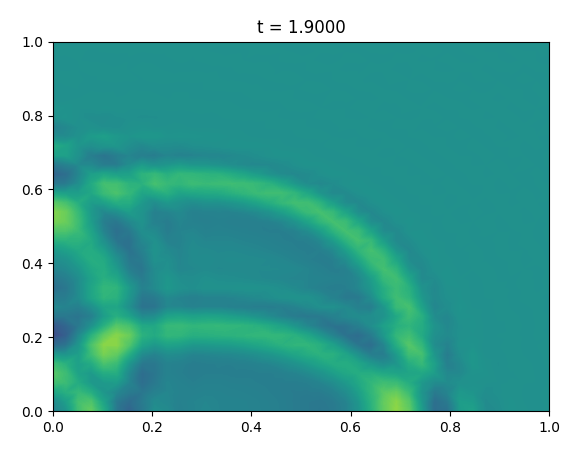
\includegraphics[width=0.5\textwidth]{figures/wave_eqn_outframe.png}
    \caption{Output of (\texttt{examples/demo\_wave\_equation.py}). A single frame of the wave equation demo code. The relevant solving code is provided in \autoref{fig:example-wave-timeloop}.}
    \label{fig:wave-eqn-frame}
\end{figure}

\subsection{Plotter}

\texttt{FastFEM} uses \texttt{PyVista}'s (insert source here) plotting capabilities for visual representation. There are currently six methods available to the user:

\begin{itemize}
    \item \texttt{define\_plotter()}: This is a helper method, responsible for interfacing the mesh object as produced by the mesher to \texttt{PyVista}'s own requirements. Notably, it returns a PyVista grid object containing all relevant information on the nodes and connectivity of the mesh, and is subsequently used for plotter generation.
    \item \texttt{plot\_mesh()}: This method is responsible for plotting the mesh object, and confirming \texttt{PyVista}'s redering is correct. In addition, it has aethetics related parameters that can be switched to the user's liking.
    \item \texttt{plot\_data()}: This method will plot the data on a mesh, without any time dependency. It is intended to either plot a single frame of the equation \ref{pde}, of its steady-state solution.
    \item \texttt{animate\_data()}: This method will plot the time-dependent data in an interactive window, such that the user can directly test the quality of their mesh/validity of their data.
    \item \texttt{make\_movie()}: This method will output a .mp4 file of the time-dependent data.
    \item \texttt{make\_gif()}: This method will output a .gif file of the time-dependent data.
\end{itemize}

Of most notable note, the interactive widnow generated by \texttt{plot\_mesh()} will strongly resemble the output as shown in figure \ref{fig:mesh}, but with higher customizability. A sample output is given in figure \ref{fig:PyVistaMesh}.

\begin{figure}[H]
    \centering
    \hfill
    \begin{subfigure}[c]{0.3\textwidth}
        \centering
        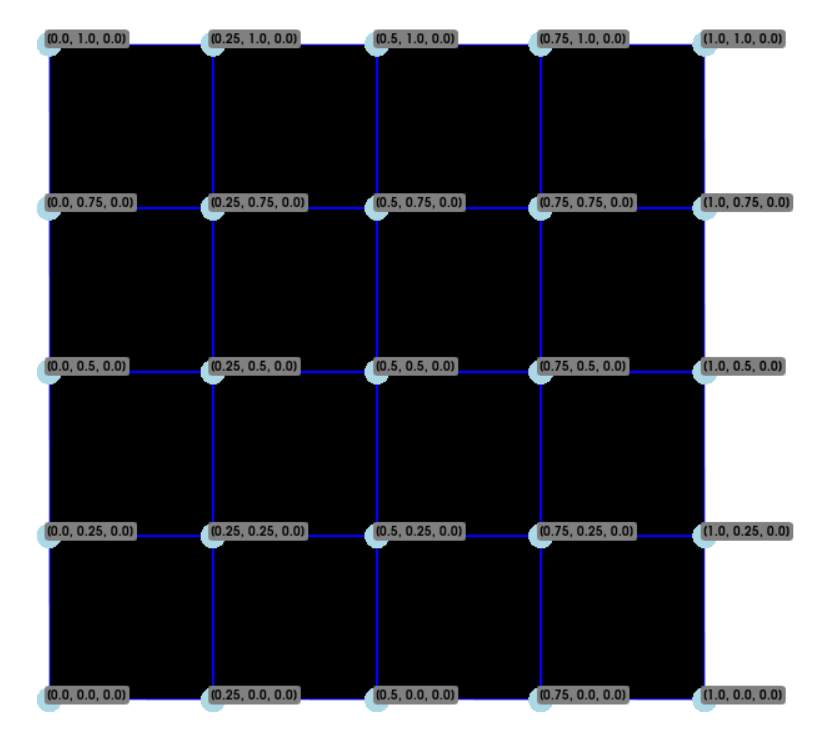
\includegraphics[width=\textwidth]{figures/PyVistaMesh_Customized.png}
        \caption{Ordered mesh, with quadrangles.}
        \label{fig:PyVistaMesh1}
    \end{subfigure}
    \hspace{0.1\textwidth}
    \begin{subfigure}[c]{0.4\textwidth}
        \centering
        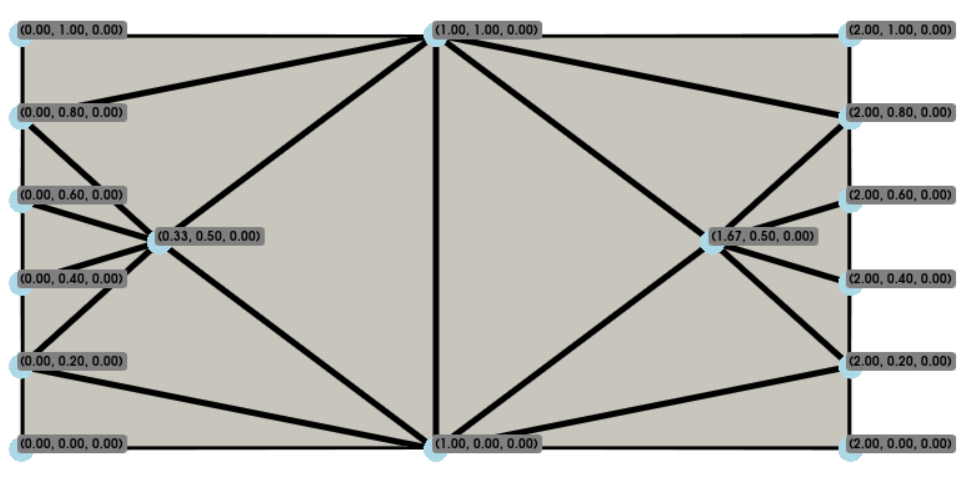
\includegraphics[width=\textwidth]{figures/PyVistaMesh_Customized2.png}
        \caption{Disordered mesh, with triangles.}
        \label{fig:PyVistaMesh2}
    \end{subfigure}
    \caption{Mesh outputs of \texttt{plot\_mesh()}, using \texttt{PyVista}'s rendering capabilities.}
    \label{fig:PyVistaMesh}
    \hfill
\end{figure}

Where the user may also interact with the mesh, and rotate it to any angle.

In addition, a single frame may also be plotted using the \texttt{plot\_data()} method, given the PDE has already been solved separately, and the content of each node in stored in a 3-dimensional array, for each time-step of the simulation. A sample output is given in figure \ref{fig:PyVistaPlotFrame}.

\begin{figure}[H]
    \centering
    \hfill
    \begin{subfigure}[c]{0.4\textwidth}
        \centering
        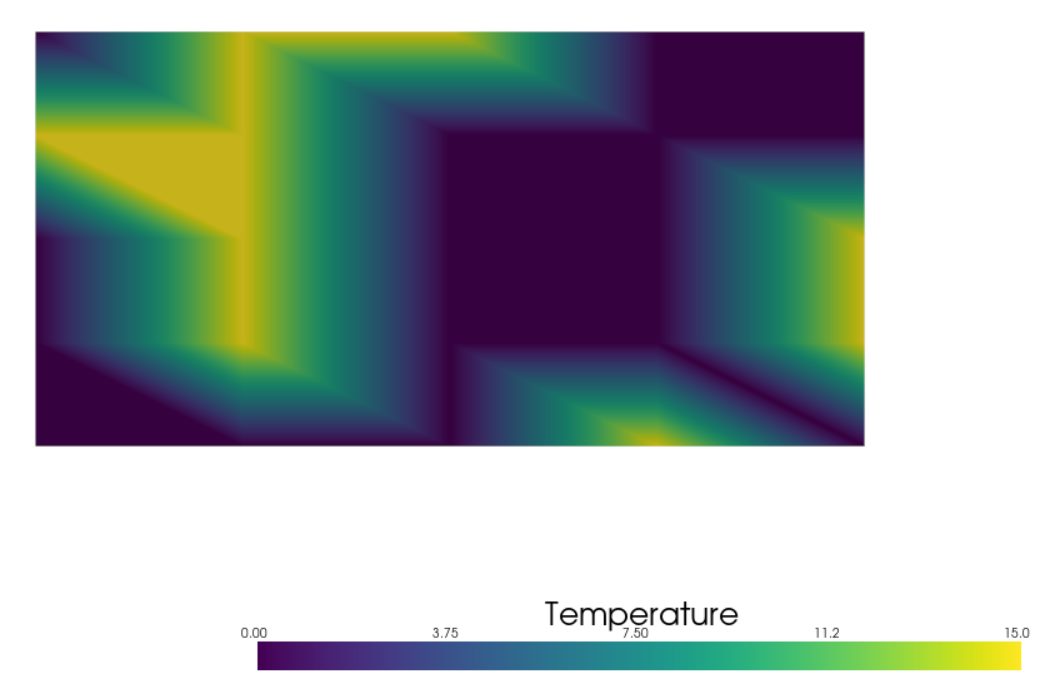
\includegraphics[width=\textwidth]{figures/PyVistaMesh_32.png}
        \caption{Plotted sample data, with 32 elements.}
        \label{fig:PyVistaMesh1}
    \end{subfigure}
    \hspace{0.1\textwidth}
    \begin{subfigure}[c]{0.4\textwidth}
        \centering
        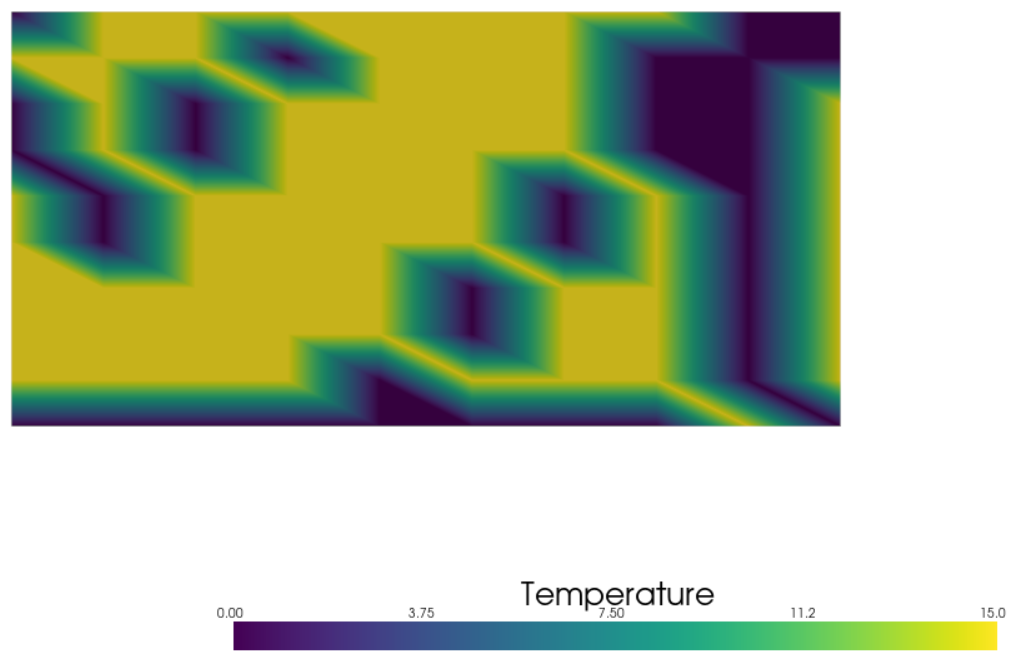
\includegraphics[width=\textwidth]{figures/PyVistaMesh_162.png}
        \caption{Plotted sample data, with 162 elements.}
        \label{fig:PyVistaMesh2}
    \end{subfigure}
    \caption{Outputs of \texttt{plot\_data()}.}
    \label{fig:PyVistaPlotFrame}
    \hfill
\end{figure}

Where the change in the number of elements accurately represents an increase in the resolution and quality of the solution.

In addition, another capability added by the \texttt{plotter} branch is the ability to animate the data interactively, and subsequently save a movie or gif of such data. A sample output is given in figure \ref{fig:PyVistaAnimated}.

\begin{figure}[H]
    \centering
    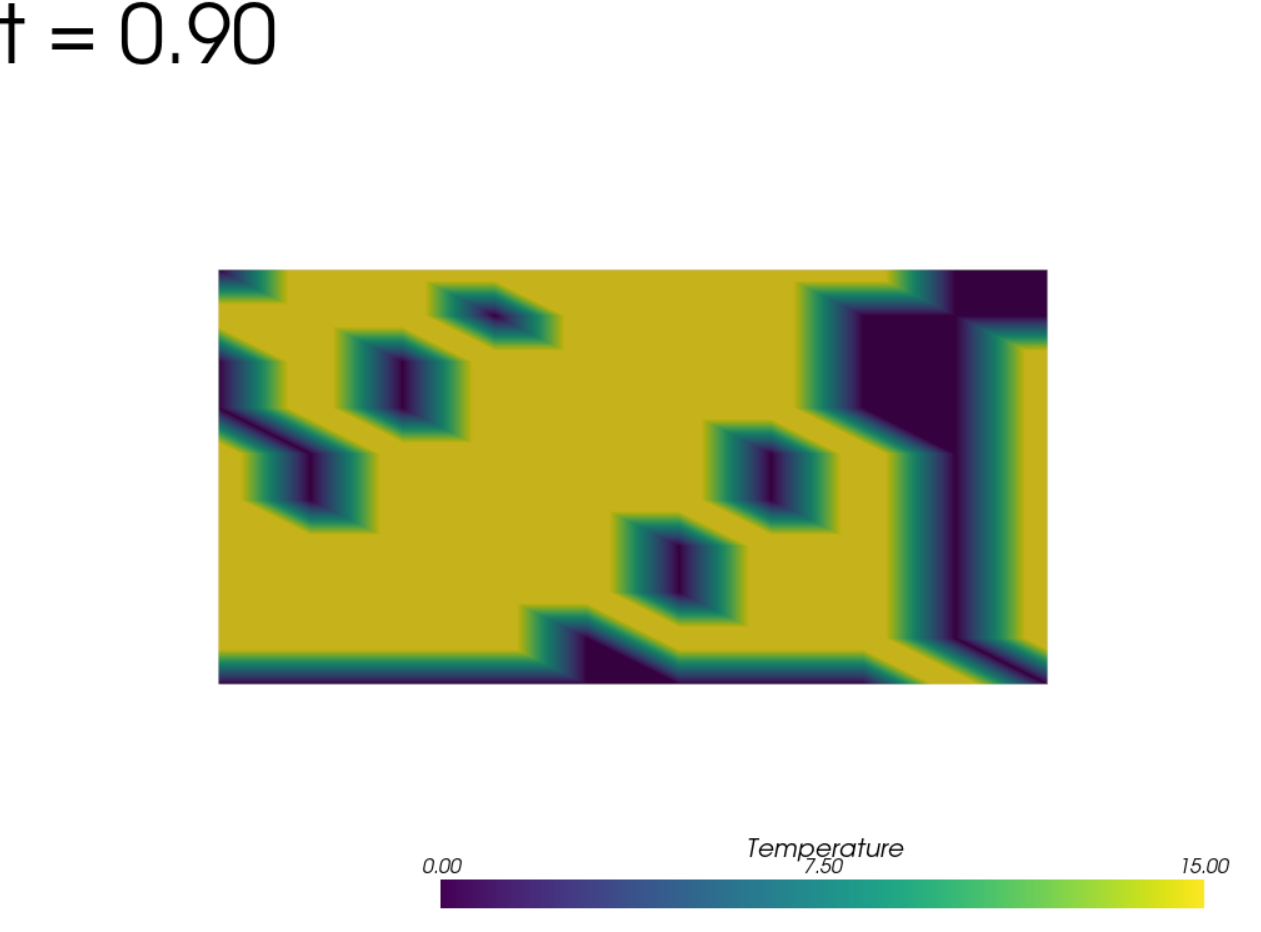
\includegraphics[width=0.5\textwidth]{figures/PyVista_Animated.png}
    \caption{A single frame of the animated data.}
    \label{fig:PyVistaAnimated}
\end{figure}

Where the most notable difference with the \texttt{plot\_data()} method is the plotted time at the top-left corner of the figure. In addition, using the \texttt{animate\_data()} method, the user has control over the number of frames per second of the animation, and enhance readability of the solution.

\textbf{Note}: Throughout the development of the \texttt{plotter} branch, testing remained a difficult aspect of the project. Many of the methods use rely on visual cues and generated plots to understand their validity. As such, the evaluation of the methods relied primarily in the assertion of the \textit{creation} of the method, rather than its actual content. To achieve this, \texttt{PyVista}'s show method (responsible for actually outputting the plot) was mocked using \texttt{unittest} and the \texttt{MonkeyPatch} testing fixture, such that no plot was actually generated thorugh the tests.

Another particular difficulty lied in the testing of the \texttt{make\_movie()} and \texttt{make\_gif()} methods, due to incompabilities of file writing across different operating systems and their reliance on external libraries, which resulted in tests passing locally but not through GitHub's CI pipeline. As such, these tests are currently skipped, while the issue is being actively debugged.




\section{Results}

\section{Software Quality and Maintenance}

\texttt{FastFEM} is open-source and version-controlled on GitHub\supercite{fastfem}. We are following some rules to ensure high software quality for better maintainability:

\begin{itemize}
    \item Direct pushes to the "main" branch are not allowed. All the contributions should be made as a pull request.
    \item Each pull request should be reviewed by two developers, and all the automated tests should be passed before it is merged.
    \item All the documentation and reports related to the software are maintained in the same repository.
    \item All the important discussions are conducted on the issues page.
    \item The changelog is kept.
    \item Semantic Versioning 2.0.0\supercite{semanticVersioning} convention is followed for versioning.
\end{itemize}

\texttt{FastFEM} also uses many other open-source tools for various reasons:
\begin{itemize}
    \item Hatch\supercite{hatch} is used as a project manager.
    \item MkDocs\supercite{mkdocs} with Material theme\supercite{mkdocsmaterial} is used for the documentation.
    \item MkDocstrings\supercite{mkdocstrings} is used to generate API references.
    \item pytest\supercite{pytest} is used to write automated tests.
    \item GitHub Actions\supercite{githubactions} is used to run the automated tests after each update.
    \item pre-commit\supercite{precommit}, Ruff\supercite{ruff}, and Black\supercite{black} are used for linting and formatting.
    \item pre-commit.ci is used to run the linters and formatters after each update.
\end{itemize}


\section{Conclusion and Outlook}

\clearpage
\printbibliography

\end{document}